\subsection{Algorithmic Learner Modeling and SR}

SR is a memory consolidation technique grounded in the psychological phenomenon of the spacing effect, which holds that information reviewed across distributed intervals is retained more durably than information reviewed in massed practice \cite{ebbinghaus1885memory, cepada2006}. Algorithmic implementations of SR automate the scheduling of these intervals by maintaining a model of each learner's memory state and adjusting review frequency accordingly. This subsection surveys the foundational algorithm underpinning aBridgeAI's learner modeling layer, its theoretical memory model, and its known limitations in institutional deployment contexts.

\subsubsection{The SM-2 Algorithm}
\label{sec:sm2_limitation}
The SuperMemo-2 (SM-2) algorithm, introduced by Wozniak in 1987 and subsequently refined \cite{wozniak1998sm2}, is among the most widely adopted SR scheduling algorithms in educational software. It introduced item-level difficulty differentiation through a scalar parameter termed the Easiness Factor ($EF$), which governs the rate at which review intervals grow for each knowledge item independently. This allowed the algorithm to adapt review schedules to the relative difficulty of individual items rather than applying a uniform spacing function across all material.

\paragraph{Interval Scheduling}
SM-2 schedules reviews through a recursive interval function. The first two intervals are fixed:
\begin{equation}
    I(1) = 1 \text{ day}, \qquad I(2) = 6 \text{ days}.
    \label{eq:sm2_base_intervals}
\end{equation}
All subsequent intervals are computed as:
\begin{equation}
    I(n) = I(n-1) \cdot EF, \quad n > 2,
    \label{eq:sm2_interval}
\end{equation}
where $EF$ is initialised at $EF_0 = 2.5$ for all items and bounded below by $EF_{\min} = 1.3$ to prevent pathologically short intervals on items of high difficulty. The interval therefore grows multiplicatively with each successful review, reflecting the empirical observation that successfully recalled items can tolerate progressively longer delays before the next review without meaningful loss of retention \cite{wozniak1998sm2}.

\paragraph{Easiness Factor Update}
After each review, $EF$ is updated according to the learner's reported 
quality response value $q \in \{0, 1, 2, 3, 4, 5\}$:
\begin{equation}
    EF_{\text{new}} = EF_{\text{old}} + 
    \left(0.1 - (5 - q)\left(0.08 + (5 - q) \cdot 0.02\right)\right).
    \label{eq:sm2_ef_update}
\end{equation}
This update rule penalises $EF$ for low $q$ values and rewards it for high $q$ values, with the neutral point at $q = 4$ producing approximately zero net change. Items recalled with difficulty accumulate lower $EF$ values and are therefore scheduled more frequently; items recalled effortlessly accumulate higher $EF$ values and are scheduled less frequently. The $EF$ floor of $1.3$ ensures that even the most difficult items eventually stabilise at a reviewable cadence rather than collapsing into daily repetition indefinitely.

\paragraph{Failure and Reset}
If $q < 3$, the item is considered failed. The interval resets to $I = 1$ day, the repetition counter returns to zero, and the item re-enters the learning queue regardless of its prior history. The $EF$ penalty is nonetheless applied, ensuring that repeated failures progressively reduce the item's interval growth rate even as the absolute interval resets.

\paragraph{Quality Response Scale}
The quality response value $q$ is the sole input the algorithm receives from the learner per review. In the original SM-2 specification, $q$ is assigned entirely through learner self-assessment after the correct answer has been revealed. The semantic definitions of each value are summarised in Table~\ref{tab:sm2_quality_scale}.

\begin{table}[H]
\centering
\small
\renewcommand{\arraystretch}{1.3}
\caption{Quality response scale used in the SM-2 SR algorithm \cite{wozniak1998sm2}.}
\begin{tabular}{|c|p{11cm}|}
\hline
\textbf{$q$} & \textbf{Response Quality Description} \\
\hline
5 & Perfect response; the correct answer is recalled immediately 
    and without effort. \\
\hline
4 & Correct response after a brief hesitation. \\
\hline
3 & Correct response recalled with noticeable difficulty. \\
\hline
2 & Incorrect response; the correct answer feels familiar upon 
    seeing it. \\
\hline
1 & Incorrect response; the correct answer is only partially 
    recognised after review. \\
\hline
0 & Complete blackout; no recognition of the correct answer 
    whatsoever. \\
\hline
\end{tabular}
\label{tab:sm2_quality_scale}
\end{table}

\paragraph{Known Limitations}
Although SM-2 has demonstrated practical effectiveness across decades of deployment in self-study tools \cite{kornell2009}, several structural limitations bear directly on its applicability in institutional learning environments.

First, the algorithm treats $q$ as a honest self-assessment, assuming the learner has no incentive to misreport. This assumption is well-founded in solo study contexts but breaks down when $q$ accumulates into metrics that influence externally visible outcomes such as lesson progression or instructor-facing dashboards.

Second, interval growth is governed solely by $EF$, which encodes only the historical pattern of $q$ values for a given item. The algorithm applies no model of item-level response demand — a brief factual question and a complex multi-step problem receive identical scheduling treatment once their $EF$ values converge, despite the substantially different cognitive effort required to answer each.

Third, SM-2 does not model the passage of time between reviews beyond the binary distinction of whether the review occurred before or after the scheduled date. A student who reviews every card one day late receives identical scheduling to one who reviews on time, and a student who never reviews an overdue card suffers no algorithmic consequence — their $EF$ remains frozen at its last recorded value indefinitely \cite{wozniak1998sm2}.

These limitations motivate the design adaptations described in Section~\ref{sec:system_sm2}, where aBridgeAI's hybrid scheduling model is specified.

\subsubsection{Memory Models: Stability and Retrievability}

Whilst SM-2 provides a practical scheduling heuristic, its interval recurrence function does not derive from an explicit model of how memory traces form, strengthen, or decay over time. A more theoretically grounded account of memory dynamics is provided by the Two-Component Model of Memory, which characterises the state of any memorised item through two independent variables: memory stability and memory retrievability \cite{wozniak1995twocomponents}.

\paragraph{The Forgetting Curve}
The empirical foundation of SR theory is Ebbinghaus's forgetting curve, first described in 1885 \cite{ebbinghaus1885}. Ebbinghaus demonstrated through systematic self-experimentation that the probability of successful recall declines as a negatively exponential function of elapsed time since the last successful review:
\begin{equation}
R(t) = e^{-\frac{t}{S}}
\end{equation}
where $R(t) \in [0, 1]$ denotes the probability of recall at time $t$ days after the last review, and $S$ denotes a stability parameter governing the rate of decay. Items with higher stability retain acceptable recall probability over longer intervals; items with lower stability decay rapidly toward chance-level performance. This formulation implies that forgetting is not a discrete event but a continuous process, and that any fixed review interval will produce different retention outcomes for items of differing stability.

\paragraph{Memory Stability}
Memory stability $S$ represents the durability of a memory trace — formally, the inter-repetition interval at which the probability of successful recall equals a target retention threshold, typically set at $R = 0.9$ \cite{wozniak1995twocomponents}. Stability is not an intrinsic property of the material alone but reflects the interaction between item difficulty, the learner's prior knowledge, and the history of prior retrievals. Each successful retrieval increases stability, a phenomenon termed the retrieval practice effect \cite{roediger2006}, with the magnitude of the stability increase depending on the retrievability at the moment of practice: retrievals attempted when recall probability is low produce larger stability gains than retrievals attempted when recall probability is high \cite{bjork1994}. This is the theoretical basis for spacing reviews at intervals that allow some forgetting to occur before the next retrieval rather than reviewing while recall is still effortless.

\paragraph{Memory Retrievability}
Memory retrievability $R$ represents the probability of successful recall at a specific point in time, computed from the forgetting curve given the current stability $S$ and the elapsed time since the last review $t$. Unlike stability, which changes only at the moment of review, retrievability decays continuously between reviews. At the moment of a successful review, retrievability resets to 1.0 and then begins declining again according to the exponential function above. Retrievability thus provides a real-time estimate of a learner's current knowledge state for any given item, independent of when the next scheduled review falls \cite{wozniak1995twocomponents}.

\paragraph{Stability Increase and the Role of Difficulty}
The Two-Component Model further specifies that the increase in stability $\Delta S$ produced by a successful retrieval is governed by an Optimum Factor ($OF$), which encodes the relationship between retrievability at the time of review and the resulting stability gain. Items reviewed at low retrievability — that is, items that the learner has nearly forgotten — yield disproportionately large stability increases, consistent with the desirable difficulties framework described by Bjork \cite{bjork1994}. This property motivates scheduling reviews near the point of forgetting rather than significantly before or after it, which is the theoretical justification for the interval lengths produced by SM-2 and its successors.

Absolute item difficulty, termed the A-Factor in SuperMemo's formulation \cite{wozniak1998sm2}, modulates stability growth independently of retrievability. High A-Factor items require more repetitions to achieve equivalent stability to low A-Factor items, reflecting genuine differences in material complexity that persist across learners. Separating item difficulty from learner-specific memory dynamics allows the model to distinguish between an item that is universally difficult and a learner who is individually struggling, a distinction that has practical consequences for both scheduling and content design.

\paragraph{Relationship to SM-2}
SM-2 can be understood as an approximation of the Two-Component Model operating without explicit stability or retrievability estimates. The Easiness Factor $EF$ functions as a proxy for stability — items with high $EF$ grow intervals rapidly, consistent with high stability — but it encodes no continuous retrievability estimate and applies no forgetting curve between reviews. The consequence is that SM-2 responds only to review outcomes, not to the passage of time between reviews. An item due for review three months ago carries the same $EF$ as the day it was last reviewed, despite the intervening decay in its true retrievability. More recent algorithms, including SM-17 and the FSRS.
\cite{ye2023fsrs}, address this by maintaining explicit stability and retrievability estimates updated continuously over time, at the cost of greater computational and parametric complexity. The theoretical properties of stability and retrievability nonetheless inform the design of aBridgeAI's learner-facing performance metrics, as described in Section~\ref{sec:system_sm2}.

\subsubsection{Knowledge Tracing and Learner Modeling}

SR algorithms model memory at the level of individual items, scheduling each card independently based on its own retrieval history. A complementary line of research, termed knowledge tracing, addresses a broader question: given a sequence of observed practice attempts, what is the probability that a learner has mastered an underlying knowledge component at any given point in time? Where SR optimises \textit{when} to review, knowledge tracing estimates \textit{whether} mastery has been achieved \cite{corbett1994}.

\paragraph{Bayesian Knowledge Tracing}
The foundational model in this field is Bayesian Knowledge Tracing (BKT), introduced by Corbett and Anderson \cite{corbett1994} in the context of the ACT programming tutor. BKT models each knowledge component as a latent binary variable — either mastered or not mastered — and updates the probability of mastery after each practice attempt using Bayes' theorem. The model is parameterised by four values:

\begin{itemize}
    \item $P(L_0)$: the prior probability that the learner has already 
    mastered the knowledge component before any practice.
    \item $P(T)$: the probability of transitioning from unmastered to 
    mastered after a single practice opportunity.
    \item $P(S)$: the probability of a slip — answering incorrectly 
    despite having mastered the component.
    \item $P(G)$: the probability of a guess — answering correctly 
    without having mastered the component.
\end{itemize}

After each observed response, the posterior probability of mastery 
$P(L_n)$ is updated as:

\begin{equation}
P(L_n \mid \text{correct}) = \frac{P(L_{n-1})(1 - P(S))}{P(L_{n-1})(1 - P(S)) + (1 - P(L_{n-1})) \cdot P(G)},
\end{equation}

\begin{equation}
P(L_n \mid \text{incorrect}) = \frac{P(L_{n-1}) \cdot P(S)}{P(L_{n-1}) \cdot P(S) + (1 - P(L_{n-1}))(1 - P(G))}.
\end{equation}

The updated posterior is then carried forward as the prior for the next practice attempt, allowing the model to track mastery probability as a continuous trajectory over the learner's practice history. A mastery threshold — typically $P(L_n) \geq 0.95$ — determines when a learner is considered to have sufficiently mastered a component and may progress \cite{corbett1994}.

BKT established several principles that remain influential in educational data mining: the separation of latent knowledge state from observed performance, the explicit modeling of slip and guess probabilities as noise sources, and the use of a mastery threshold as a progression gate. However, BKT operates on discrete knowledge components modeled independently, with no mechanism for capturing relationships between components or for modeling the continuous decay of knowledge over time \cite{pardos2010}.

\paragraph{Deep Knowledge Tracing}
Piech et al. \cite{piech2015dkt} extended knowledge tracing to sequence modeling using recurrent neural networks, introducing Deep Knowledge Tracing (DKT). Rather than maintaining an explicit probability for each knowledge component, DKT encodes the learner's entire interaction history as a hidden state vector within a long short-term memory (LSTM) network, and predicts the probability of correct response on any future knowledge component from this compressed representation. This allows the model to implicitly capture relationships between knowledge components — for instance, that mastery of TCP flow control is predictive of performance on TCP congestion control — without requiring these relationships to be explicitly specified by a domain expert.

DKT demonstrated substantially improved predictive accuracy over BKT on large-scale educational interaction datasets \cite{piech2015dkt}, and subsequent variants have incorporated attention mechanisms, graph structures, and forgetting functions to further improve performance \cite{pandey2019}. However, DKT and its successors require substantial interaction data to train reliably, operate as largely opaque models offering limited interpretability, and are computationally intensive relative to the closed-form updates of BKT or SM-2 \cite{khajah2016}.

\paragraph{Per-Student State Isolation}
A principle common to both BKT and SM-2 is that knowledge state is modeled at the level of the individual learner. Each student maintains an independent set of parameters — mastery probabilities in BKT, Easiness Factors in SM-2 — that evolve according to their own practice history without influence from peer performance. This isolation is not merely a computational convenience but a theoretical necessity: the same observable response pattern may reflect different underlying knowledge states in different learners depending on their prior experience, learning strategies, and domain familiarity \cite{corbett1994, vanlehn2006}. Aggregating or sharing state across learners would systematically misrepresent individual knowledge trajectories and undermine the validity of any progression gate derived from the model.

This principle of per-student state isolation is directly adopted in aBridgeAI's learner modeling design, as elaborated in Section~\ref{sec:system_sm2}.

\paragraph{Item-Level Demand and Latency Normalisation}
A challenge in using raw response latency as a cognitive signal is that observed latency confounds retrieval effort with item-level reading and processing demand. A learner responding to a lengthy, multi-clause technical question will necessarily exhibit higher latency than a learner responding to a brief factual question, regardless of their underlying memory state for the relevant knowledge. Meaningful interpretation of response latency therefore requires normalisation against an item-specific baseline that accounts for the inherent processing demand of the question itself \cite{cowan2001}.

Several approaches to this normalisation have been proposed in the literature. Standardisation against population response time distributions — dividing individual latency by the mean or median latency for that item across all learners — removes item-level demand while preserving individual differences in retrieval speed. Where population data is unavailable, item-level demand can be estimated from surface features of the stimulus: reading time models based on word count and syntactic complexity provide principled baselines against which individual latency can be compared. Technical content specifically warrants a conservative reading rate estimate, as domain-specific vocabulary and conceptual density slow comprehension relative to general prose. Difficulty ratings assigned by domain experts provide a further adjustment factor, capturing the additional cognitive demand imposed by items that require not only reading but active problem construction or multi-step reasoning \cite{Cog2019Sweller}.

\paragraph{Response Time in Automated Assessment}
The use of response time as a formal scoring input in automated assessment systems has gained traction alongside the growth of computer-based testing. Item Response Theory extensions incorporating response time — most notably the hierarchical model of van der Linden \cite{vanderlinden2007} — treat latency as a second observed variable alongside accuracy, jointly informing estimates of both item difficulty and learner ability. In adaptive learning systems, response time has been used to adjust item selection, to detect disengaged or random responding, and to calibrate difficulty estimates in the absence of sufficient historical response data \cite{lee2014}. These applications share the common principle that response latency, when properly normalised, provides diagnostic information about the learner's cognitive state that accuracy-only models systematically discard.

The theoretical basis established here — that normalised response latency reflects memory strength beyond what correctness alone captures, and that item-level demand must be accounted for in any latency-based signal — directly motivates the expected time formulation and $Q$ derivation model specified in Section~\ref{sec:q_derivation}.

\begin{figure}[H]
\centering
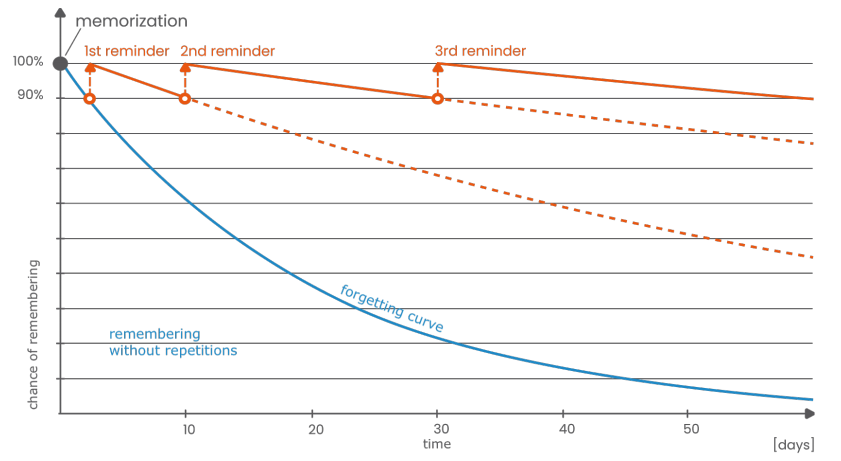
\includegraphics[width=1\textwidth]{graphics/introduction/forgetting_curve.png}
\caption{Forgetting curves applied in SR learning. Source: \cite{pokrywka2023lstm_srs}.}
\label{fig:forgetting_curve}
\end{figure}
